\documentclass[12pt,a4paper]{article}
\usepackage[top=2cm,left=1cm,right=1cm,bottom=2cm]{geometry}
\usepackage{amssymb,mathtools,amsthm}
\usepackage{fourier}
\usepackage{xcolor}
\usepackage{multicol, array, fancyhdr}
\usepackage{tikz}
\usetikzlibrary{angles,quotes}
\usepackage{tasks}
\newcommand{\Lim}{\displaystyle\lim}
\renewcommand{\columnseprule}{1pt}
\renewcommand{\arraystretch}{1.5}
\newcommand{\vect}{\overrightarrow}
\newcommand{\lin}{\overline}
\newcommand{\R}{\mathbb{R}}
\newcommand{\s}{\sin}
\newcommand{\cs}{\cos}
% \renewcommand{\dfrac}[2]{\displaystyle\dfrac{#1}{#2}}


%======================================================
\newtheoremstyle{mystyle}
  {\topsep}% espace avant
  {\topsep}% espace après
  {\upshape}% police du corps du théorème
  {}% indentation (vide pour rien, \parindent)
  {\bfseries\sffamily}% police du titre du théorème
  { :}% ponctuation après le théorème
  { }% après le titre du théorème (espace ou \newline)
  {%
    \rule[0.5\baselineskip]{0.5\textwidth}{1pt}%
    \newline\fcolorbox{black}{white}{%
      \thmname{#1}\thmnumber{ \textup{#2}}\thmnote{ \textnormal{(#3)}}%
    }%
    
    % \vspace{0.5em} % Adjust vertical space after the title
  }% spécifications du titre

\theoremstyle{mystyle}
\newtheorem{exo}{Exercice}

%======================================================



\begin{document}


\pagestyle{fancy}
\fancyhf{} % clear all header and footer fields
\fancyhead[L]{Lycée : Zitoun \hspace{1.5cm} Année scolaire : 2024-2025} % Left header
\fancyhead[C]{ \hspace{4cm} Niveau : TCS} % Right-Center header
\fancyhead[R]{Prof. Othmane Laksoumi} % Right header
\fancyfoot[C]{\thepage} % Footer


\begin{center}
    \textbf{\Large Calcul trigonométrique }
\end{center}
\begin{multicols*}{2}

\begin{exo}
\text{ }
\begin{enumerate}
    \item Convertir en radian les mesures suivantes : \\\(15^\circ\) ; \(100^\circ\) ; \(172^\circ\) ; \(400^\circ\) ; \(500^\circ\) ; \(2025^\circ\)
    
    \item Convertir en degré les mesures suivantes : \\\(\dfrac{\pi}{9}\) ; \(\dfrac{\pi}{12}\) ; \(\dfrac{\pi}{15}\) ; \(\dfrac{5\pi}{9}\) ; \(\dfrac{3\pi}{4}\) ; \(\dfrac{11\pi}{12}\)
\end{enumerate}
\end{exo}

\begin{exo}
On considère la figure ci-contre,
\begin{center}
	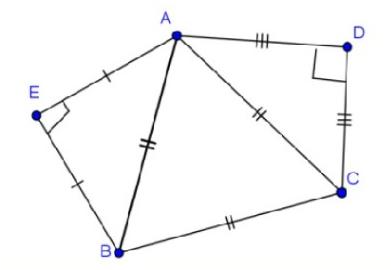
\includegraphics[scale=0.5]{Exercice2}
\end{center}
Donner la mesure principale de chacun des angles orientés suivants :

\[
\left( \overline{\overrightarrow{AB}, \overrightarrow{AC}} \right) ; \left( \overline{\overrightarrow{DC}, \overrightarrow{AC}} \right) ; \left( \overline{\overrightarrow{CB}, \overrightarrow{CD}} \right)
\]
\[
\left( \overline{\overrightarrow{EB}, \overrightarrow{EA}} \right) ; \left( \overline{\overrightarrow{BC}, \overrightarrow{EB}} \right) ; \left( \overline{\overrightarrow{AB}, \overrightarrow{AD}} \right)
\]
\end{exo}

\begin{exo}
Soit \( ABC \) un triangle dans le plan tel que : \( \left( \overline{\overrightarrow{AB}, \overrightarrow{AC}} \right) \equiv \alpha [2\pi] \). Calculer en fonction de \( \alpha \) les mesures des angles orientés suivants :
\[
\left( \overline{\overrightarrow{AC}, \overrightarrow{AB}} \right) ; \left( \overline{\overrightarrow{BA}, \overrightarrow{AC}} \right) ; \left( \overline{\overrightarrow{CA}, \overrightarrow{BA}} \right) \text{ et } \left( \overline{\overrightarrow{CA}, \overrightarrow{AB}} \right)
\]
\end{exo}

\begin{exo}
Soient \( \vect{U}, `\vect{V}, \vect{W} \) et \( \vect{K} \) des vecteurs dans le plan tels que :
\[
\left( \lin{\vect{U}, \vect{V}} \right) = \dfrac{\pi}{2} [2\pi] ; \left( \lin{\vect{W}, \vect{V}} \right) = -\dfrac{\pi}{3} [2\pi] ; \left( \lin{\vect{K}, \vect{W}} \right) = \dfrac{\pi}{4} [2\pi]
\]
Déterminer les mesures de l'angle orienté \( \left(\lin{\vect{U}, \vect{K}}\right) \).
\end{exo}
\newcolumn
\begin{exo}
\text{ }
\begin{enumerate}
	\item Calculer $\cos(x)$ et $\tan(x)$ sachant que :\\ $\sin(x) = \dfrac{\sqrt{2}}{3}$ et $\dfrac{\pi}{2} < x < \pi$.
	\item Calculer $\cos(x)$ et $\sin(x)$ sachant que :\\ $\tan(x) = 2\sqrt{3}$ et $-\pi < x < -\dfrac{\pi}{2}$.
	\item Calculer $\cos(x)$ et $\tan(x)$ sachant que :\\ $\tan(x) = \sqrt{3} - \sqrt{2}$ et $x\in]-\pi;0[$.
	\item Calculer $\sin(x)$ et $\tan(x)$ sachant que :\\ $\cos(x) = -\dfrac{3}{4}$ et $-\pi < x < 0$.
	
	
\end{enumerate}

\end{exo}

\begin{exo}
Soit $x\in\R$.
\begin{enumerate}
	\item Montrer que : $$(\cos(x) + \sin(x))^2 + (\cos(x) - \sin(x))^2 = 2$$
	\item On suppose que : $\cos(x) - \sin(x) = \sqrt{2}$.
		\begin{enumerate}
			\item Montrer que $\cos(x) + \sin(x) = 0$
			\item Déduire les valeurs de $\cos(x)$ et $\sin(x)$.
		\end{enumerate}
\end{enumerate}
\end{exo}

\begin{exo}
Simplifier les expression suivantes :
\begin{enumerate}
	\item $A = (\cos(x) + \sin(x))^2 - (\cos(x) - \sin(x))^2$
	\item $B = \cos^4(x) - \sin^4(x) + \sin^2(x) - \cos^2(x)$
	\item $C = \sin^4(x) - \cos^4(x) + 2\cos^2(x)$
%	\item $D = \sin^6(x) + \cos^6(x) + \cos^4(x) + \sin^4(x) + 5\sin^2(x)\cos^2(x)$
\end{enumerate}
\end{exo}

\begin{exo}
Soit $x\in\R$ tel que : $\cos(x)\neq 0$.\\Montrer que :
\begin{enumerate}
	\item 
		\begin{enumerate}
			\item $\tan^2(x) - \sin^2(x) = \tan^2(x).\sin^2(x)$
			\item Déduire que : $\sin^2(x) = \dfrac{\tan^2(x)}{1 + \tan^2(x)}$
		\end{enumerate}
	\item $\dfrac{\s^2(x) - \s^4(x)}{\cs^2(x) - \cs^4(x)} = 1$
%	\item 
\end{enumerate}
\end{exo}
\newpage
\begin{exo}
Soit $x$ un nombre réel.
\begin{enumerate}
	\item Simplifier : \\$\s(30\pi + x)$ ; $\cs(400\pi + x)$ ; $\s(3\pi + x)$ ; $\cs(51\pi + x)$ ; $\s(17\pi - x)$ ; $\cs(45\pi - x)$ ; $\s(102\pi + x)$ ; $\cs(40\pi + x)$.
	\item Simplifier : \\$\s\left(\dfrac{\pi}{2} + x\right)$ ; $\cs\left(\dfrac{\pi}{2} + x\right)$ ; $\s\left(\dfrac{3\pi}{2} + x\right)$ ; $\cs\left(\dfrac{51\pi}{2} - x\right)$
\end{enumerate}
\end{exo}

\begin{exo}
Soit $x\in\R$. Simplifier :\\ \\
%\begin{enumerate}
	 $A = \s\left(\dfrac{\pi}{2} + x\right) + \cs\left(\dfrac{5\pi}{2} - x\right) + \s(5\pi - x) - \cs(3\pi - x)$
	 $B = \cs\left(\dfrac{\pi}{2} - x\right) - \s(x + 3\pi) + \cs\left(\dfrac{3\pi}{2} - x\right) + \s(\pi - x)$
\end{exo}

\begin{exo}
Soit $x$ un nombre réel de l'intervalle $\left[-\dfrac{\pi}{2};\dfrac{\pi}{2}\right]$.\\
Soit $A(x) = \s(x)(\cs^2(x) - \s^2(x))$
\begin{enumerate}
	\item Calculer $A(0), A\left(\dfrac{\pi}{4}\right),A\left(\dfrac{\pi}{3}\right), A\left(\dfrac{\pi}{6}\right)$ et $A\left(\dfrac{5\pi}{6}\right)$.
	\item Montrer que : $A\left(\dfrac{\pi}{2} - x\right) = A\left(\dfrac{\pi}{2} + x\right).$
\end{enumerate}
\end{exo}

\begin{exo}
Soit $x$ un nombre réel de l'intervalle $\left[-\dfrac{\pi}{2};\dfrac{\pi}{2}\right]$.\\
Soit $A(x) = \dfrac{1}{2}\left[(\cs^2(2x) - \s^2(2x)) - 1\right]$
\begin{enumerate}
	\item Calculer $A\left(\dfrac{\pi}{4}\right)$ et $A\left(-\dfrac{\pi}{8}\right)$.
	\item Montrer que : $A(x) = \s(2x)\cs(2x)$.
	\item Montrer que : $A(-x) = -A(x)$
	\item Calculer : $A(x) + A\left(x + \dfrac{\pi}{4}\right)$
\end{enumerate}
\end{exo}

\begin{exo}
Résoudre dans $]-\pi;\pi]$ les équations et les inéquations suivantes :\\
$\bullet \cs(x) = \dfrac{\sqrt{3}}{2} \ \ \ \bullet 2\cs(x) + \sqrt{2} = 0 \ \ \ \bullet\cs\left(x + \dfrac{\pi}{4}\right) = \dfrac{1}{2}$\\
$\bullet \cs(x) \geq \dfrac{\sqrt{3}}{2} \ \ \ \bullet 2\cs(x) + \sqrt{2} < 0 \ \ \ \bullet\cs\left(x + \dfrac{\pi}{4}\right) \leq \dfrac{1}{2}$
\end{exo}

\begin{exo}
Résoudre dans $]0,2\pi]$ les équations et les inéquations suivantes :\\
%\begin{itemize}
     $\bullet\sin(x) = \dfrac{\sqrt{2}}{2}$
     $\bullet2\sin(x) + \sqrt{3} = 0$
     $\bullet\sin(x) = \cos\left(\dfrac{\pi}{3}\right)$
     $\bullet\sin(x) \geq \dfrac{1}{2}$
     $\bullet2\sin(x) + \sqrt{3} < 0$
     $\bullet\sin(x) = \cos\left(\dfrac{\pi}{8}\right)$
%\end{itemize}
\end{exo}

\begin{exo}
Résoudre dans $]-\dfrac{\pi}{2}, \dfrac{\pi}{2}[$ les équations et les inéquations suivantes :\\
%\begin{itemize}
     $\bullet\tan(x) = \sqrt{3}$
     $\bullet\tan\left(x + \dfrac{\pi}{3}\right) + 1 = 0$
     $\bullet\tan(x) > \sqrt{3}$
     $\bullet\tan\left(x + \dfrac{\pi}{3}\right) > 0$
%\end{itemize}
\end{exo}

\begin{exo}
Soit $x$ un nombre réel.\\On pose : $A(x) = 2\cos^2(x) + \sin(x) - 1$.
\begin{itemize}
    \item[a)] Calculer $A\left(\dfrac{\pi}{6}\right)$.
    \item[b)] Vérifier que : $A(x) = (1 - \sin(x))(1 + 2\sin(x))$.
    \item[c)] Résoudre dans $\mathbb{R}$ l'équation $A(x) = 0$.
\end{itemize}
\end{exo}

\begin{exo}
Résoudre les équations suivantes dans l'intervalle $I$ :
\begin{itemize}
    \item $2\cos^2(x) - \cos(x) = 0$, $I = ]-\pi,\pi]$
    \item $\sin^2(x) - \sin(x) = 0$, $I = ]-\pi,\pi]$
    \item $2\cos^2(x) - 3\cos(x) = 0$, $I = ]-2\pi,\pi]$
    \item $\sin^2(x) - 3\sin(x) = 0$, $I = ]-\pi,\pi]$
    \item $\tan^2(x) - \sqrt{3}\tan(x) = 0$, $I = ]-\dfrac{\pi}{2},\dfrac{\pi}{2}[$
\end{itemize}
\end{exo}




\end{multicols*}



\end{document}
